%!TEX root = ../main.tex 

\section{Comment une impédance?}

\subsection{Matching à la source}

\begin{frame}{Matching à la source}
    \begin{itemize}
        \item Plupart des circuits avec sortie CMOS
        \item $Z_o \rightarrow 0\Omega$
    \end{itemize}
    \begin{columns}
        \begin{column}{0.25\textwidth}
            \begin{center}
                \begin{figure}
                \centering
                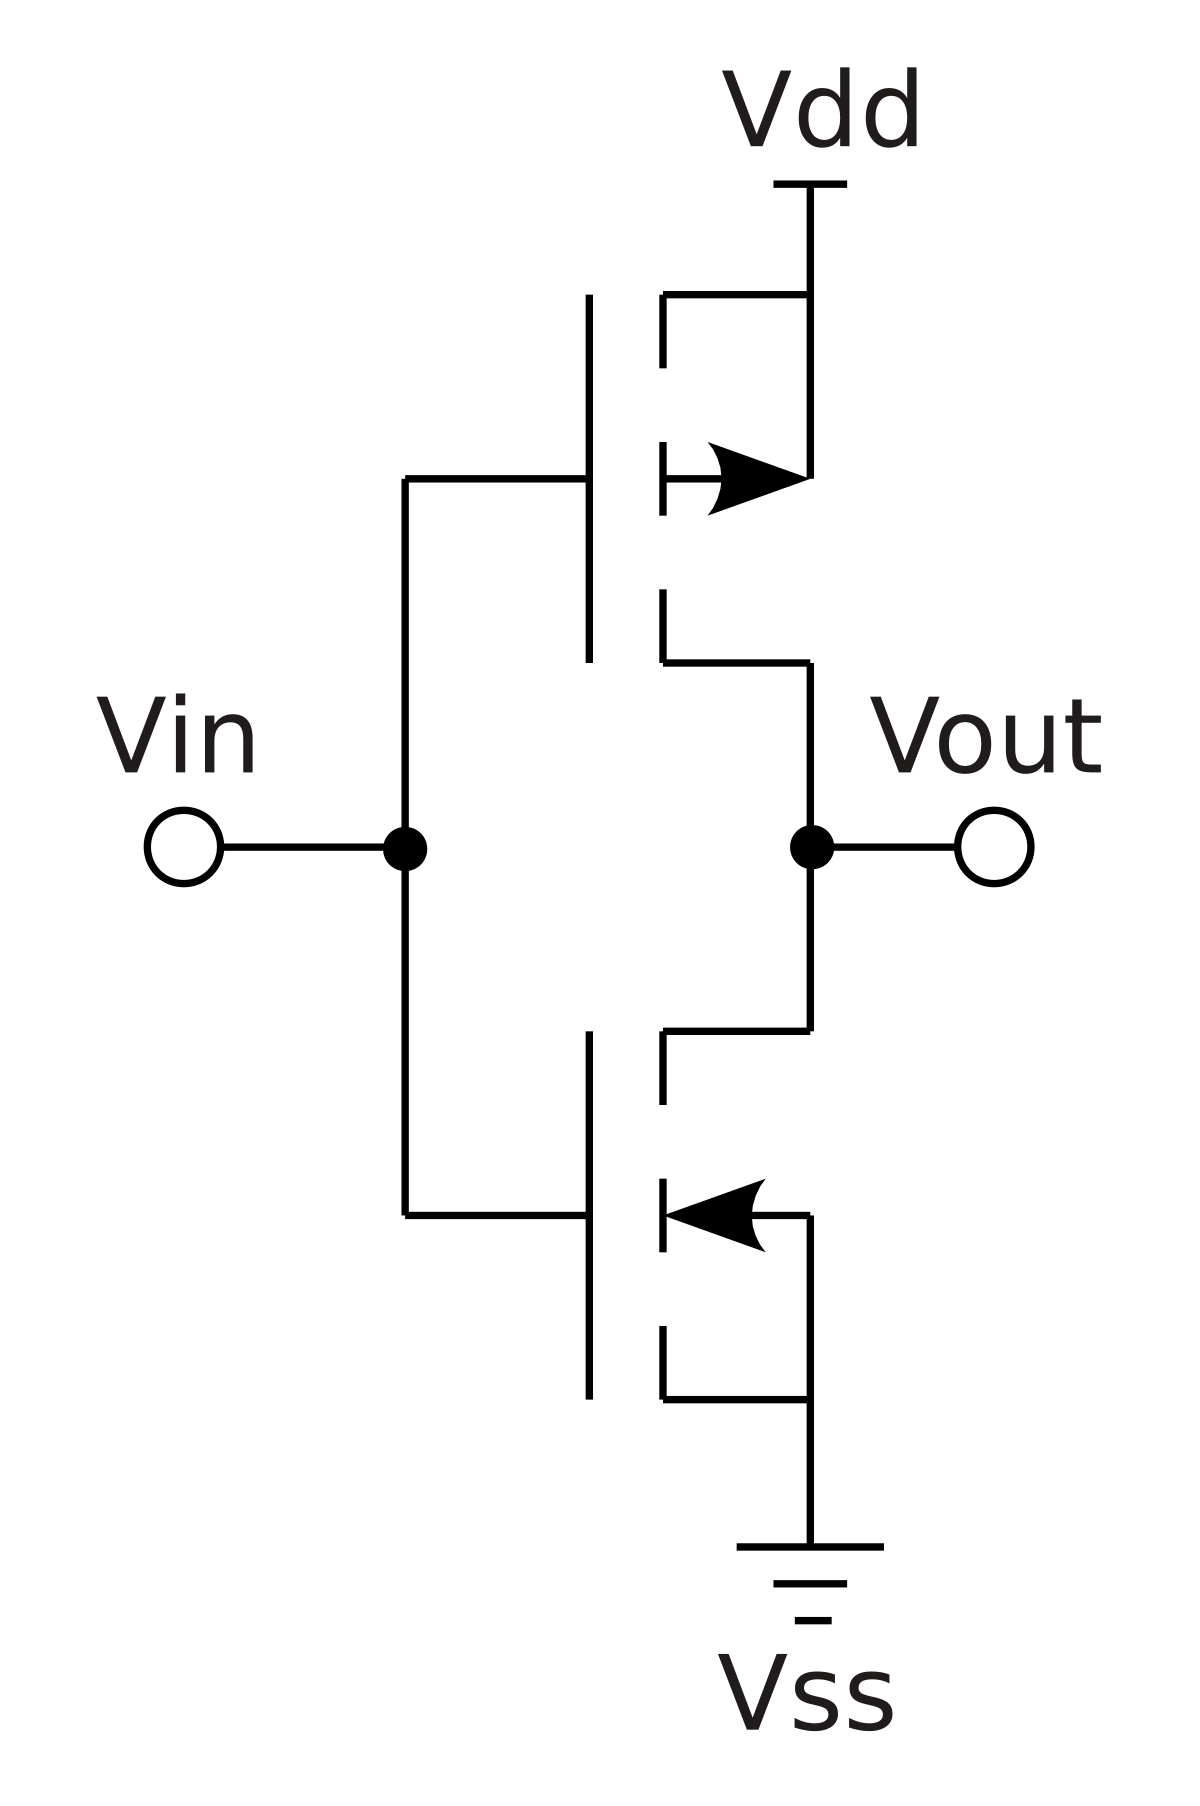
\includegraphics[width=\textwidth]{pictures/CMOS_inverter.png}
            \end{figure}
            \end{center}
        \end{column}
        \begin{column}{0.75\textwidth}
            \begin{center}
                \resizebox{\textwidth}{!}{
                \ctikzset{bipoles/resistor/height=0.1}
                \ctikzset{bipoles/resistor/width=0.3}
                \begin{circuitikz}[american voltages]
                    \draw [thick]
                    (0,0) to [short, *-] (10,0)
                    to [european resistor, l=$Z_L$] (10, 4)
                    (0,0) to [open, v<=$V_S$] (0,4)
                    to [short, *-] (1, 4)
                    to [amp, a=$Z_o \rightarrow 0$] (3, 4)
                    to [short] (6, 4)
                    to [european resistor, l=$Z_0$] (8, 4)
                    to [short] (10,4)
                    ;
                    \draw
                    (0, 0) to [open] (1.25, 4)
                    to [R] (2.75, 4)
                    ;
                \end{circuitikz}
                }
            \end{center}
        \end{column}
    \end{columns}
\end{frame}

\begin{frame}{Matching à la source - Résistance série}
    \begin{columns}
        \begin{column}{0.3\textwidth}
            \begin{itemize}
                \item Ajouter une résistance externe!
                \item Très proche de la sortie
                \bigskip
                \item Valider $Z_o$ du IC
                \item $Z_S = Z_0 - Z_o$
            \end{itemize}
        \end{column}
        \begin{column}{0.7\textwidth}
            \begin{center}
            \resizebox{\textwidth}{!}{
            \ctikzset{bipoles/resistor/height=0.1}
            \ctikzset{bipoles/resistor/width=0.3}
            \begin{circuitikz}[american voltages]
                \draw [thick]
                (0,0) to [short, *-] (10,0)
                to [european resistor, l=$Z_L$] (10, 4)
                (0,0) to [open, v<=$V_S$] (0,4)
                to [short, *-] (1, 4)
                to [amp, a=$Z_o \rightarrow 0$] (3, 4)
                to [european resistor, l=$Z_S$, color=red] (5, 4)
                to [short] (6, 4)
                to [european resistor, l=$Z_0$] (8, 4)
                to [short] (10,4)
                ;
                \draw
                (0, 0) to [open] (1.25, 4)
                to [R] (2.75, 4)
                ;
            \end{circuitikz}
            }
            \end{center}
        \end{column}
    \end{columns}
\end{frame}


\subsection{Matching à la load}

\begin{frame}{Matching à la load}
    \begin{itemize}
        \item Plupart des circuits avec entrée CMOS
        \item $Z_L \rightarrow \infty\Omega$
    \end{itemize}
    \begin{columns}
        \begin{column}{0.25\textwidth}
            \begin{center}
                \begin{figure}
                \centering
                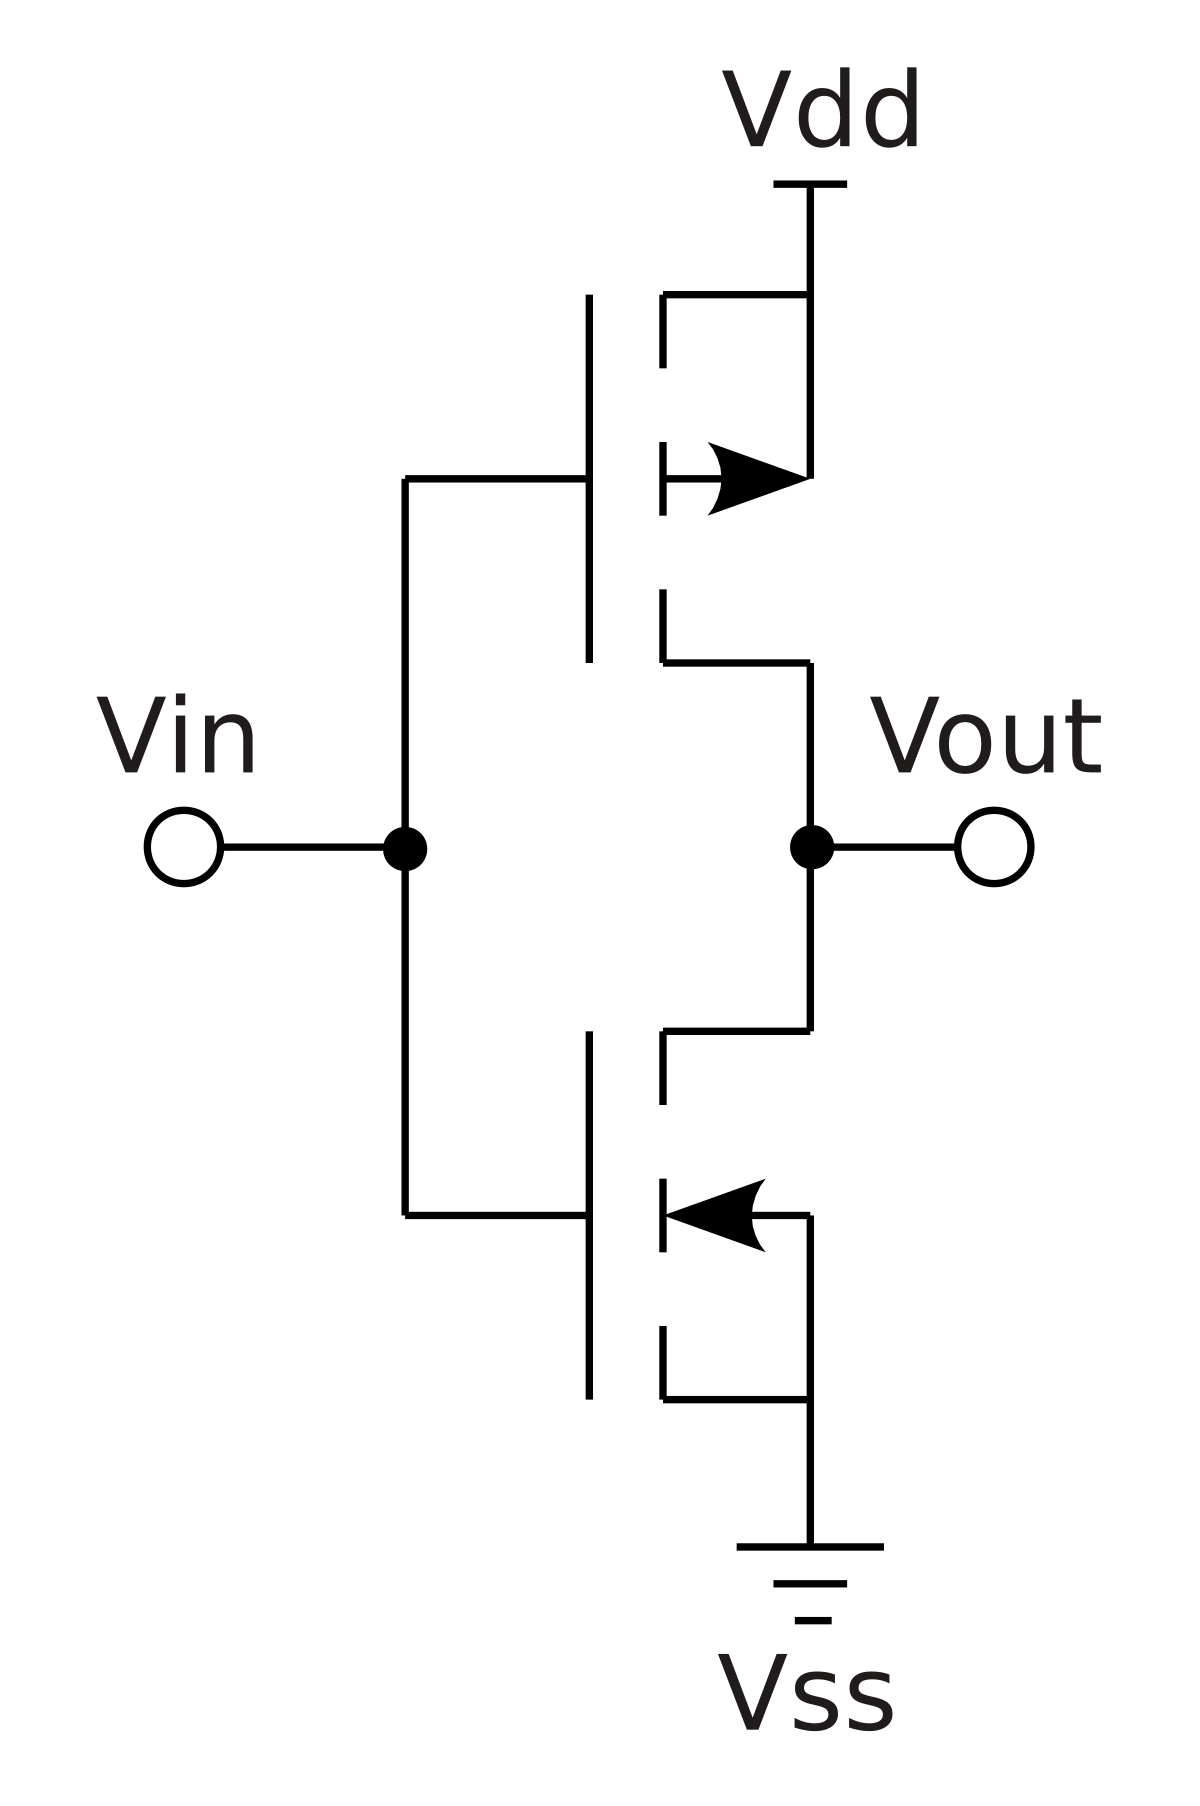
\includegraphics[width=\textwidth]{pictures/CMOS_inverter.png}
            \end{figure}
            \end{center}
        \end{column}
        \begin{column}{0.75\textwidth}
            \begin{center}
                \resizebox{\textwidth}{!}{
                \ctikzset{bipoles/resistor/height=0.1}
                \ctikzset{bipoles/resistor/width=0.3}
                \begin{circuitikz}[american voltages]
                    \draw [thick]
                    (0,0) to [short, *-] (10,0)
                    to [open] (10, 4)
                    (0,0) to [open, v<=$V_S$] (0,4)
                    to [short, *-] (1, 4)
                    to [amp, a=$Z_o \rightarrow 0$] (3, 4)
                    to [european resistor, l=$Z_S$] (4.25, 4)
                    to [european resistor, l=$Z_0$] (7, 4)
                    to [amp, a=$Z_i \rightarrow \infty$] (10, 4)
                    ;
                    \draw
                    (0, 0) to [open] (1.25, 4)
                    to [R] (2.75, 4)
                    ;
                \end{circuitikz}
                }
            \end{center}
        \end{column}
    \end{columns}
\end{frame}

\begin{frame}{Matching à la load - Résistance parallèle}
    \begin{columns}
        \begin{column}{0.3\textwidth}
            \begin{itemize}
                \item Ajouter une résistance externe!
                \item Très proche de l'entrée
                \bigskip
                \item Valider $Z_i$ du IC
                \item $Z_L = Z_0 - \frac{Z_0}{Z_i}$
            \end{itemize}
        \end{column}
        \begin{column}{0.7\textwidth}
            \begin{center}
            \resizebox{\textwidth}{!}{
            \ctikzset{bipoles/resistor/height=0.1}
            \ctikzset{bipoles/resistor/width=0.3}
            \begin{circuitikz}[american voltages]
                \draw [thick]
                    (0,0) to [short, *-] (10,0)
                    to [open] (10, 4)
                    (0,0) to [open, v<=$V_S$] (0,4)
                    to [short, *-] (1, 4)
                    to [amp, a=$Z_o \rightarrow 0$] (3, 4)
                    to [european resistor, l=$Z_S$] (4.25, 4)
                    to [european resistor, l=$Z_0$] (7, 4)
                    to [amp, a=$Z_i \rightarrow \infty$] (10, 4)
                    ;
                \draw [thick]
                    (7.5, 4) to [european resistor, l=$Z_L$, color=red] (7.5, 0)
                    ;
                \draw
                    (0, 0) to [open] (1.25, 4)
                    to [R] (2.75, 4)
                    ;

            \end{circuitikz}
            }
            \end{center}
        \end{column}
    \end{columns}
\end{frame}

\subsection{Matching du conducteur}

\begin{frame}{Impédance caractéristique}
    \begin{itemize}
        \item L'impédance caractéristique $Z_0$ d'une ligne de transmission
        \item Ne dépend que de la \textit{géométrie} de la ligne de transmission
        \item Contrôle les éléments capacitifs et inductifs parasites, qui dominent
        \bigskip
        \item Augmenter largeur de trace $\rightarrow$ plus de capacitance
        \item Augmenter distance entre les traces $\rightarrow$ plus d'inductance
        \bigskip
        \item \textit{Dans un PCB, l'inductance parasite domine toujours!}
    \end{itemize}
\end{frame}

\begin{frame}{Géométries}
    \begin{center}
        \begin{figure}
            \centering
            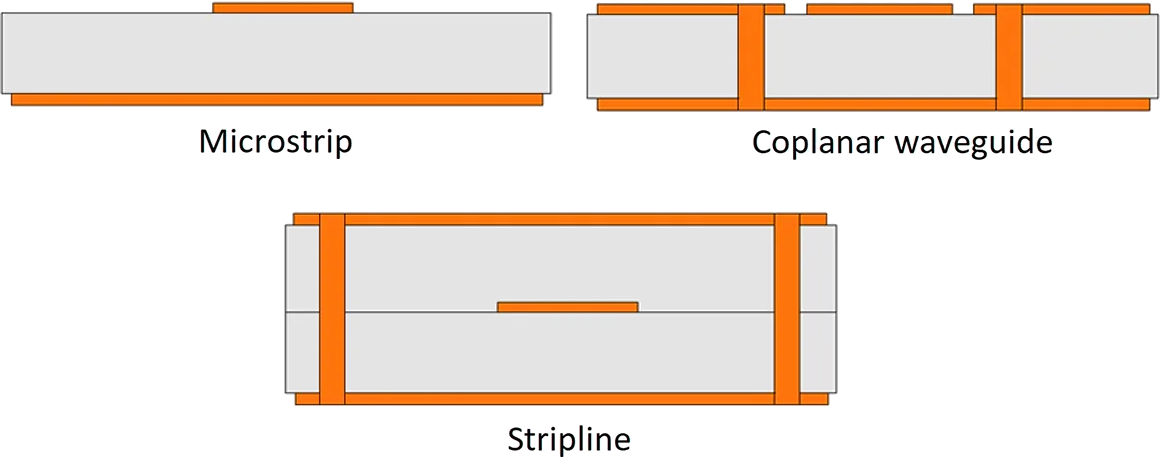
\includegraphics[width=\textwidth]{pictures/microstrip-VS-Stripline-vs-coplanar-waveguide.png}
        \end{figure}
    \end{center}
\end{frame}

\begin{frame}{Microstrip}
    \begin{columns}
        \begin{column}{0.66\textwidth}
            \begin{itemize}
                \item Trace sur le TOP / BOTTOM du PCB
                \item Plan de retour en-dessous de la trace
                \item Diélectrique d'un seul côté
                \bigskip
                \item Signal plus rapide
                \item EMI
            \end{itemize}
        \end{column}
        \begin{column}{0.33\textwidth}
            \begin{center}
                \begin{figure}
                    \centering
                    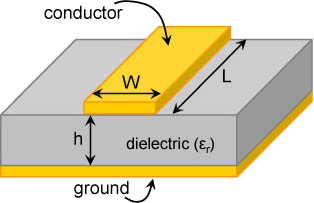
\includegraphics[width=\textwidth]{pictures/microstrip.png}
                \end{figure}
            \end{center}
        \end{column}
    \end{columns}
\end{frame}

\begin{frame}{Microstrip - Formule}
    \begin{itemize}
        \item Norme IPC-2141
        \item Approximation empirique
    \end{itemize}
    \pause
    \begin{center}
        \[
            Z_0 =
            \begin{cases} 
                \dfrac{60}{\sqrt{\varepsilon_{eff}}}\ln\left(8\frac{H}{W} + 0.25\frac{W}{H}\right), & \text{if } \frac{W}{H} < 1 \\
                \dfrac{120 \pi}{\sqrt{\varepsilon_{eff}} \cdot \left(\frac{W}{H} + 1.393 + \frac{2}{3}\ln\left(\frac{w}{H} + 1.444\right)\right)}, & \text{if } \frac{W}{H} \geq 1
            \end{cases}
        \]
        \[
            \varepsilon_{eff} \coloneqq
            \begin{cases} 
                \frac{\varepsilon_r + 1}{2} + \frac{\varepsilon_r - 1}{2} \cdot \left(\left(1 + 12 \frac{H}{W}\right)^{-\frac{1}{2}} + 0.04\left(1 - \frac{W}{H}\right)^2\right), & \text{if } \frac{W}{H} < 1 \\
                \frac{\varepsilon_r + 1}{2} + \frac{\varepsilon_r - 1}{2} \cdot \left(1 + 12 \frac{H}{W}\right)^{-\frac{1}{2}}, & \text{if } \frac{W}{H} \geq 1
            \end{cases}
        \]
    \end{center}
\end{frame}

\begin{frame}{Microstrip - Calculs}
    \begin{columns}
        \begin{column}{0.5\textwidth}
            \begin{itemize}
                \item Utiliser des calculateurs en ligne
                \item Dimensions des la trace
                \begin{itemize}
                    \item Largeur
                    \item Épaisseur métal
                    \item Distance au plan
                    \item Constante diélectrique $\varepsilon$
                    \item Gap entre métaux
                \end{itemize}
            \end{itemize}
        \end{column}
        \begin{column}{0.5\textwidth}
            \begin{figure}
                \centering
                
\includegraphics[width=\textwidth, height=0.33\textwidth, keepaspectratio]{pictures/altium.png}
            \end{figure}
            \vspace{-12pt}
            \begin{figure}
                \centering
                
\includegraphics[width=\textwidth, height=0.33\textwidth, keepaspectratio]{pictures/kicad.png}
            \end{figure}
        \end{column}
    \end{columns}

    \begin{figure}
        \centering
        
\includegraphics[width=\textwidth, height=0.2\textwidth, keepaspectratio]{pictures/saturn-pcb.png}
    \end{figure}
\end{frame}

\begin{frame}{Stripline}
    \begin{columns}
        \begin{column}{0.6\textwidth}
            \begin{itemize}
                \item Trace sur une couche interne du PCB
                \item Plan de retour de chaque bord de la trace
                \item Diélectrique des deux côtés
                \bigskip
                \item Signal plus lent
                \item Moins de radiation
            \end{itemize}
        \end{column}
        \begin{column}{0.4\textwidth}
            \begin{center}
                \begin{figure}
                    \centering
                    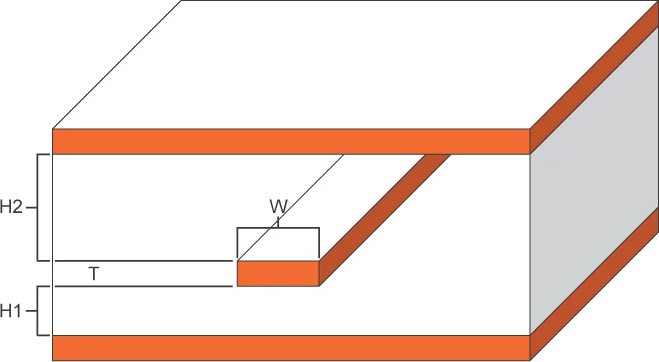
\includegraphics[width=\textwidth]{pictures/stripline.png}
                \end{figure}
            \end{center}
        \end{column}
    \end{columns}
\end{frame}

\subsection{Impédance Différentielle}

\begin{frame}{Paire Différentielle}
    \begin{columns}
        \begin{column}{0.6\textwidth}
            \begin{itemize}
                \item Paire de signal inverse envoyés ensemble
                \item Affectés par le bruit également
                \item Annulent leur bruits respectifs
                \bigskip
                \item Impédance Single-Ended
                \item Impédance Différentielle
            \end{itemize}
        \end{column}
        \begin{column}{0.4\textwidth}
            \begin{center}
                \begin{figure}
                    \centering
                    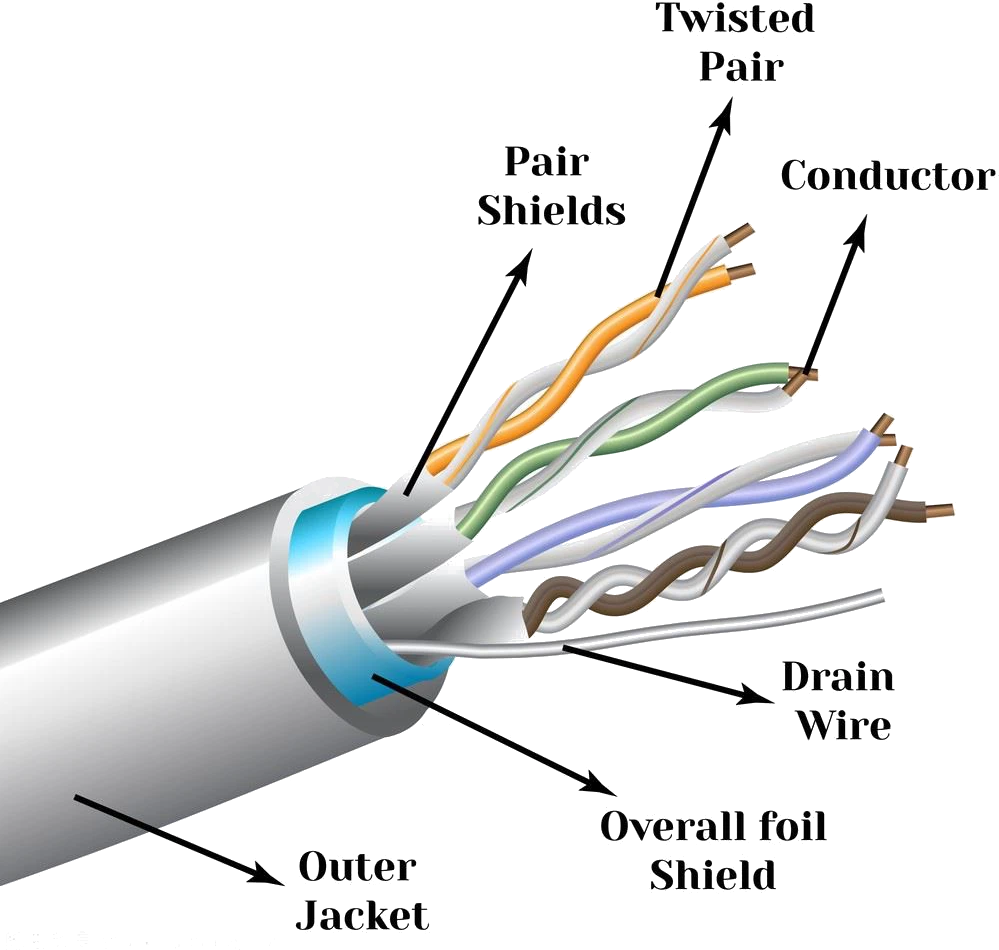
\includegraphics[width=\textwidth]{pictures/twisted-pair.png}
                \end{figure}
            \end{center}
        \end{column}
    \end{columns}
\end{frame}

\begin{frame}{Paire Différentielle}
    \begin{center}
        \resizebox{!}{0.75\textheight}{
        \begin{circuitikz}[american voltages]
            \draw [thick]
            (0,0) to [short] (10,0)
            to [european resistor, l=$Z_L$, a=$50\Omega$, color=red] (10, -4);

            \draw [thick]
            (0,0) to [american voltage source, v=$V_S$, invert] (0, 4)
            to [short] (4, 4)
            to [european resistor, l=$Z_0$, a=$50\Omega$] (6, 4)
            to [short] (10, 4)
            to [european resistor, l=$Z_L$, a=$50\Omega$] (10, 0);
            
            \draw [thick]
            (0,0) to [american voltage source, v=$V_S$, invert, color=red] (0, -4)
            to [short] (4, -4)
            to [european resistor, l=$Z_0$, a=$50\Omega$, color=red] (6, -4)
            to [short] (10, -4);

            \draw[thick, dashed]
            (8, -3.5) 
              .. controls (8.5, -1) and (8.5, 1)
              ..node[currarrow, sloped,  allow upside down, pos=1] {}
            (8, 3.5)
            ;
            \draw
            (8, 0) to [open, l={\large$100\Omega$}] (8.25, 4);

        \end{circuitikz}
        }
    \end{center}
\end{frame}

\begin{frame}{Guides d'onde différentiels}

    \begin{itemize}
        \item Il y a deux impédances à prendre en compte!
        \begin{itemize}
            \item Single-Ended
            \item Differential
        \end{itemize}
        \item Differential = $2 \cdot$ Single-Ended
        \item Géométries différentes
    \end{itemize}

    \begin{columns}
        \begin{column}{0.5\textwidth}
            \begin{center}
                \begin{figure}
                    \centering
                    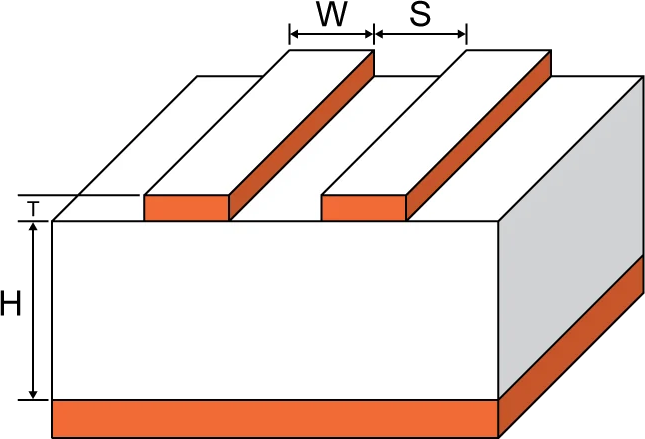
\includegraphics[width=\textwidth]{pictures/differential-microstrip.png}
                \end{figure}
            \end{center}
        \end{column}

        \begin{column}{0.5\textwidth}
            \begin{center}
                \begin{figure}
                    \centering
                    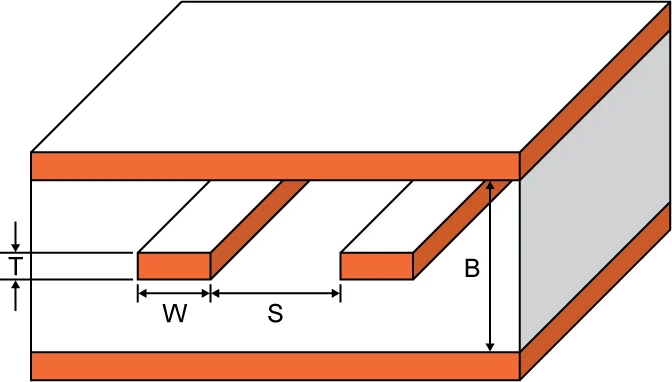
\includegraphics[width=\textwidth]{pictures/differential-stripline.png}
                \end{figure}
            \end{center}
        \end{column}
    \end{columns}
\end{frame}

\subsection{Résumé}

\begin{frame}{Impédance \& Réactance}
    \begin{columns}
        \begin{column}{0.6\textwidth}
            \begin{itemize}
                \item Impédance
                \begin{itemize}
                    \item Composé de résistance et de réactance
                    \item Résistance à une certaine fréquence
                \end{itemize}
            \end{itemize}
            \begin{center}
                $Z = \sqrt{R^2 + (X_L - X_C)^2}$
            \end{center}

            \vspace{18pt}

            \begin{itemize}
                \item<2-> Réactance
                \begin{itemize}
                    \item Résistance à une certaine fréquence
                    \item Emmagasine l'énergie dans les champs
                    \item Déphasage
                \end{itemize}
                \begin{center}
                    $X_C = \dfrac{1}{2 \pi f C}$\\
                    \vspace{10pt}
                    $X_L = 2 \pi f L$
                \end{center}
            \end{itemize}
        \end{column}
        \begin{column}{0.4\textwidth}
            \begin{center}
                \begin{figure}
                    \centering
                    \includegraphics<1->[width=\textwidth]{pictures/impedance.png}
                \end{figure}
                \begin{figure}
                    \centering
                    \includegraphics<2->[width=\textwidth]{pictures/reactance-phase.png}
                \end{figure}
            \end{center}
        \end{column}
    \end{columns}
\end{frame}

\begin{frame}{Ligne de transmission}
    \begin{columns}
        \begin{column}{0.66\textwidth}
            \begin{itemize}
                \item Tout circuit a des composants parasitiques
                \item Impédance caractéristique $Z_0$
                \item Ratio tension/courant se déplaçant
                \item Dépend de la \textit{géométrie} du circuit
            \end{itemize}
        \end{column}

        \begin{column}{0.33\textwidth}
            \begin{center}
                $Z_0 = \sqrt{\dfrac{R + j \omega L}{G + j \omega C}}$\\
                \vspace{12pt}
                $Z_0 = \sqrt{\dfrac{L}{C}}$
            \end{center}
        \end{column}
        
    \end{columns}
    \vfill
    \begin{center}
        \resizebox{0.75\textwidth}{!}{
        \begin{circuitikz}[american voltages]
            \draw [thick]
            (0,0) to [short, *-] (10,0)
            to [R, l_=$R_{LOAD}$] (10,5)
            (0,0) to [open, v<=$V$] (0,5)
            to [short, *- ,i=$i$] (2,5)
            to [R, l_=$R$] (4, 5)
            to [short] (7, 5)
            to [american inductor, l_=$L$] (9, 5)
            to [short] (10,5)
            (0, 5) to [open] (4.5, 5)
            to [C, l_=$C$] (4.5, 0)
            (0, 5) to [open] (6, 5)
            to [R, l_=$G$] (6, 0)
            ;
        \end{circuitikz}
        }
    \end{center}
\end{frame}

\begin{frame}{Réflection de signal}
    \begin{columns}
        \begin{column}{0.65\textwidth}
            \begin{itemize}
                \item Lorsque $Z_0 \neq Z_S \neq Z_L$
                \begin{itemize}
                    \item Pas assez de courant peut passer
                    \item Trop de courant est demandé
                \end{itemize}
            \end{itemize}

            \vfill
            \vspace{18pt}
            \begin{center}
                \animategraphics[autoplay, controls, loop, width=\linewidth]{12}{pictures/partial-reflection/partial-reflection-}{0}{51}
            \end{center}
        \end{column}

        \begin{column}{0.4\textwidth}
                \resizebox{\textwidth}{!}{
                \begin{circuitikz}[american voltages]
                    \draw [thick]
                    (0,0) to [short, *-] (8,0)
                    to [resistor, l=$Z_L$] (8, 4)
                    (0,0) to [open, v<=$V_S$] (0,4)
                    to [short, *-] (0.5, 4)
                    to [R, l=$Z_S$] (2.5, 4)
                    to [short] (4, 4)
                    to [european resistor, l=$Z_0$] (6, 4)
                    to [short] (8,4)
                    ;
                    \draw [thick, dashed]
                    (3, 0.5)
                      .. controls (3.5, 1) and (3.5, 3)
                      ..node[currarrow, sloped,  allow upside down, pos=1] {}
                    (3, 3.5) 
                    ;
                    \draw
                    (4, 0) to [open, l=$V$] (4.25, 4);
                \end{circuitikz}
                }

                \vfill
                \vspace{50pt}

            \begin{center}
                $\Gamma = \dfrac{Z_L - Z_0}{Z_L + Z_0}$\\
            \end{center}
        \end{column}
    \end{columns}
\end{frame}

\begin{frame}{Réflection de signal}
    \begin{figure}
        \centering
        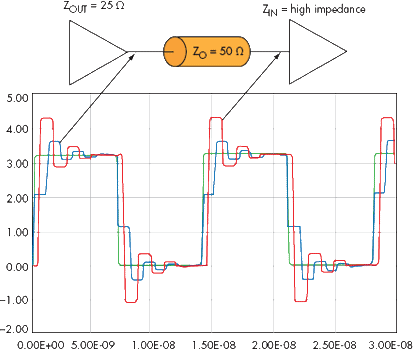
\includegraphics[width=\textwidth, height=0.8\textheight, keepaspectratio]{pictures/signal-reflection.png}
    \end{figure}
\end{frame}

\begin{frame}{Matching d'impédance}

    \begin{columns}
        \begin{column}{0.66\textwidth}
            \begin{itemize}
                \item 3 Impédances à prendre en compte
                \item Source \& Load
                \begin{itemize}
                    \item Rajouter une résistance en série
                    \item Rajouter une résistance en parallèle
                \end{itemize}
                \item $Z_0$ du conducteur
                \begin{itemize}
                    \item Contrôler la géométrie
                    \item Impédance différentielle 
                \end{itemize}
            \end{itemize}
        \end{column}
        \begin{column}{0.33\textwidth}
            \begin{figure}
                \centering
                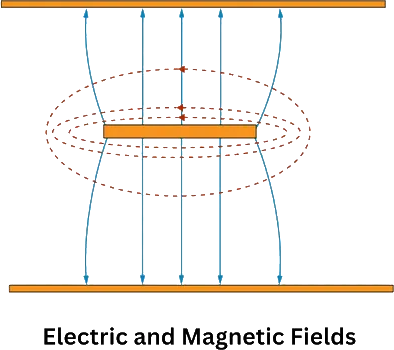
\includegraphics[width=\textwidth]{pictures/stripline-fields.png}
            \end{figure}
        \end{column}
    \end{columns}

    \vspace{-8pt}

    \begin{center}
        \resizebox{!}{0.4\textheight}{
        \ctikzset{bipoles/resistor/height=0.1}
        \ctikzset{bipoles/resistor/width=0.3}
        \begin{circuitikz}[american voltages]
            \draw [thick]
                (0,0) to [short, *-] (10,0)
                to [open] (10, 4)
                (0,0) to [open, v<=$V_S$] (0,4)
                to [short, *-] (1, 4)
                to [amp, a=$Z_o \rightarrow 0$] (3, 4)
                to [european resistor, l=$Z_S$, color=red] (4.25, 4)
                to [european resistor, l=$Z_0$] (7, 4)
                to [amp, a=$Z_i \rightarrow \infty$] (10, 4)
                ;
            \draw [thick]
                (7.5, 4) to [european resistor, l=$Z_L$, color=red] (7.5, 0)
                ;
            \draw
                (0, 0) to [open] (1.25, 4)
                to [R] (2.75, 4)
                ;

        \end{circuitikz}
        }
    \end{center}
\end{frame}